\documentclass[a4paper,10pt,twocolumn]{article}
\usepackage{lmodern}
\usepackage[english]{babel}
\usepackage[T1]{fontenc}
\usepackage[utf8]{inputenc}
\usepackage{graphicx}
\usepackage{float}
\usepackage[top=0.5cm,bottom=2cm,left=1cm,right=1cm]{geometry}
\usepackage{amsmath}
\usepackage{amssymb}

\title{Similarity of Mass Spectra}
\date{\today}
\author{Ondřej Podsztavek, podszond@fit.cvut.cz}

\begin{document}

\maketitle

\section{Project Description}

The goal of this project is to create an application which searches
in database of protein sequences for peptide sequences similar to input
mass spectra.

\subsection{Input}

Applicaiton inputs are mass spectra and database of protein
sequences.

\subsection{Ouput}

Output it set of peptide sequences similar to input mass
spectra sorted according to similarity.

\section{Solution Method}

To measure similarity, feature vectors from fearute space \(\mathbb{U}\)
and similarity measure \(\delta: \mathbb{U} \times \mathbb{U} \to \mathbb{R}\)
are needed.

Each mass spectrum is set of a peptide fragments intensities. In order to create
feature vector, easy feature extraction method is applied. Mass spectrum
intensities are binned to equal-width bins.

Protein sequences are splitted into peptides according to rule that the
sequence is splitted after occurence of amino acid 'K' or 'R' if it is not
followed by amino acid 'P'. Modified peptides from splitted peptides are
ignored and that mass spectrum for them is calcutated based on b-ionts with
charge 1. Intesities corresponding to obtained mass spectra are set to 1.
For more information please refer to~\cite{novak2009}.

Cosine similarity is chosen as similarity function. It computes the
L2-normalized dot product of vectors. That is, if \(x\) and \(y\) are vectors,
their cosine similarity \(\text{SIM}_{\cos}\) is defined as:

\[ \text{SIM}_{\cos}(x, y) = \frac{x^Ty}{\|x\|\|y\|} \]

\section{Implementation}

The application is divided into 4 modules:

\begin{itemize}
    \item mass spectra database operations,
    \item mass spectra preprocessing
    \item similarity measure,
    \item web application.
\end{itemize}

Programming language used is Python~3.6. From libraries the application requires
scikit-learn~0.19.1~\cite{scikit-learn}, NumPy~1.13.3,
SciPy~1.0.0~\cite{scipy}, Flask~0.12.2 and
pyteomics~3.4.2~\cite{Goloborodko2013}. Web application database is MongoDB.

\subsection{Database Module}

The LIL (list of lists) sparse matrix stores one list per row with entries
containing the colun index and the value. It is good format for incremental
construction.

\subsection{Similarity Module}

The similarity measure module contains the \(k\) nearest neighbour query 
(\(k\)NN). The query return matrix of indexes to database of size
\(n \times k\) where \(n\) is the number of mass spectra queried.
Row \(i\) contains indexes to most similar spectra in database in
descending order.

Cosine similarity is computed using function \texttt{cosine\_similarity}
from scikit-learn library. Its inputs are two LIL sparse matrices and output
is CSR sparse matrix. Sparse matrices are used because the feature vector
contains a lot of zero value and are difficult to srote in memory.

\subsection{Preprocessing Module}

\subsection{Web Application}

\section{Output Example}

Figure~\ref{fig:sample} shows an example result page for a spectrum with 
one similar spectrum found.

\begin{figure}[H]
    \begin{center}
        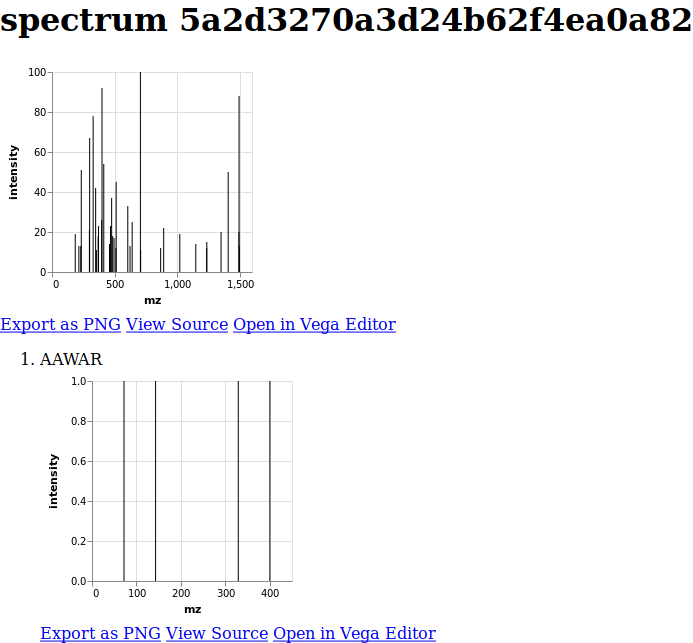
\includegraphics[width=6cm]{img/output-sample}
    \end{center}
    \caption{Flask application result page example.}
    \label{fig:sample}
\end{figure}

\section{Experiments}

For kNN query the results are following. Write about the data used.

\begin{table}[H]
    \begin{center}
        \label{table:TODO}
        \begin{tabular}{l|rrr}
            & \multicolumn{3}{c}{\textbf{bin size}} \\
            \textbf{accuracy measure} & 0.1 & 0.5 & 1 \\
            \hline
            top 1 & 6.12 & 6.37 & 6.50 \\
            top 5 & 7.46 & 8.09 & 8.22 \\
            top 10 & 8.29 & 8.80 & 8.86 \\
        \end{tabular}
        \caption{
            Accuracy of similarity search in percents for different bin sizes.
            Top 10 accuracy measures if the searched peptide sequence is between
            the first 10 returned results. Accordingly are defined the top 5
            and top 1 accuracies.
        }
    \end{center}
\end{table}

\section{Discussion}

Discuss problems of this project. For example y-ionts and a-ionts.
Range query, which will not improve accuracy.

\section{Conclusion}

This project goal was to implement application for similarity search in
database of protein sequences for peptides according to its mass spectrum.
Experiments section presents unsatisfactory results but generally the problem
of searching for similar peptides from mass spectra is hard due to nosie and
imperfection during mass spectra retrieval.

\bibliography{report}{}
\bibliographystyle{plain}

\end{document}
